\documentclass[utf8,twocolumn]{article}
\usepackage{ctex}
\usepackage{amsmath}
\usepackage{circuitikz}
\usepackage{tikz}
\usepackage{graphicx}
\usepackage{hyperref}
\usepackage{geometry}
\usepackage{pdfpages}
\usepackage{booktabs}
\usepackage{subfigure}
\usepackage{float}
\usepackage{amsmath}
\usepackage{amssymb}
% math font
\usepackage{mathrsfs}
\usepackage{multirow}
\usepackage{inputenc}
\usepackage{fancyhdr}

\title{示波器上万花尺的设计}
\author{
    jamescsq47 \\
    \texttt{chensq23@mails.tsinghua.edu.cn}
\and
    FHYQ-Dong \\
    \texttt{donghy23@mails.tsinghua.edu.cn}
}
\date{\zhtoday}

\geometry{a4paper, scale=0.8}
\setlength{\columnsep}{20pt}
\pagestyle{fancy}
\fancyhf{}
\renewcommand{\headrulewidth}{0.5pt}
\renewcommand{\footrulewidth}{0.5pt}
\lhead{示波器上万花尺的设计}
\rhead{jamescsq47~~~FHYQ-Dong}
\cfoot{---~\thepage~---}

\hypersetup{
    colorlinks=true,
    linkcolor=black,
    filecolor=black,      
    urlcolor=black,
    citecolor=black,
}


\begin{document}

\maketitle
\thispagestyle{fancy}



\section{实验设计}
\subsection{实验原理分析}
实验的预期结果是在示波器(XY模式)上显示内旋轮线。内旋轮线的参数方程如下:
\begin{equation}
\begin{aligned}
    x\left(t\right) &= \left(1 - d\right) \cos\left(2\pi f_1 t\right) + d \sin\left(2\pi f_2 t\right) \\
    y\left(t\right) &= \left(1 - d\right) \sin\left(2\pi f_1 t\right) + d \cos\left(2\pi f_2 t\right)
\end{aligned}
\end{equation}
根据内旋轮线的参数方程,需要两路频率不同的正弦模拟信号,为保证图形不转动,频率最好是严格整数比,因此采用振荡器和分频器产生频率精确的正弦信号,之后两路信号分别通过移相器产生两组相位差为$90^\circ$的信号,再交叉互换通过加法器得到要求的X信号和Y信号。


\subsection{理论结果}
设计频率比为3:4,$ d = 0.5 $。使用函数画图软件进行画图,得到理论图案如图~\ref{plot:theory_plot}。
\begin{figure}[H]
    \centering
    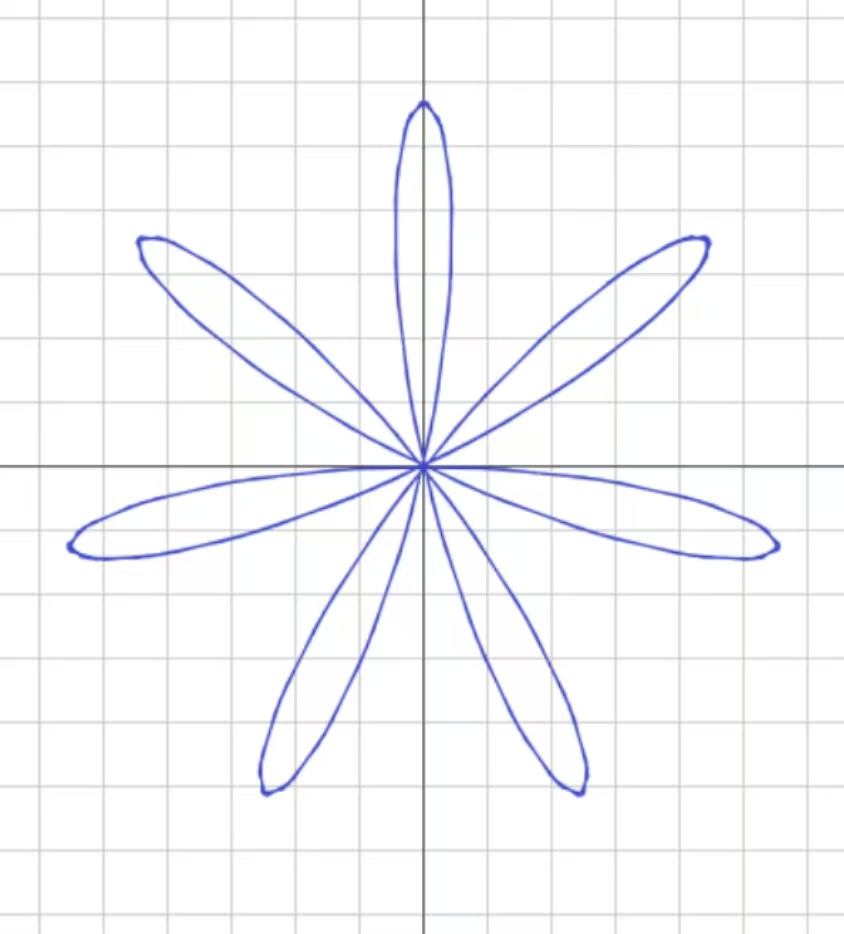
\includegraphics[width=0.6\linewidth]{images/baseline.jpg}
    \caption{频率比3:4的理论结果}
    \label{plot:theory_plot}
\end{figure}
如果正余弦函数有相位差会导致图案旋转一个角度,但仍是稳定的,不会旋转。


\subsection{总体方案设计}
电路总共分为5个模块,分别是振荡器,分频器,滤波器,移相器和加法器。其中滤波器,移相器和加法器均有2个。
\begin{itemize}
    \item \textbf{振荡器:}使用施密特触发器产生方波信号。
    \item \textbf{分频器:}将基频进行6分频和8分频。
    \item \textbf{滤波器:}采用文氏电桥滤波器结构,在实验中调节电位器,使得放大系数调至略小于3,实现滤波功能。
    \item \textbf{移相器:}将信号移相90度。
    \item \textbf{加法器:}采用运放加法电路,将移相前后的两路信号相加。
\end{itemize}


\subsection{模块具体分析}
\subsubsection{振荡器}
振捣器采用施密特触发器,电路图如图~\ref{circ:oscillator}。
\begin{figure}[H]
    \centering
    \scalebox{0.8}{
        \begin{circuitikz}[american voltages]
    \ctikzset{resistors/scale=0.5}
    \draw (0,0) to[inline schmitt] (2,0) to[short] (2,1.5) to[R, l_=$ R $] (0,1.5) to[short] (0,0);
    \draw (0,1.5) to[short] (-1,1.5) to[C, l_=$ C $] (-1,0) to[short] (-1,0) node[ground]{};
    \draw (2,0) to[short, -o] (3,0) node[right]{$ v_{out} $};
\end{circuitikz}
    }
    \caption{振荡器电路图}
    \label{circ:oscillator}
\end{figure}
其原理为电容C未充电时,施密特触发器输出高电平,通过电阻R给电容C充电,当电压超过一定阈值时,输出翻转,电容C通过电阻R放电,当电压低于一定阈值时,输出翻转,如此循环。实验使用CD40106b芯片作为施密特触发器,当 $ R = 10~\mathrm{k}\Omega $,$ C = 0.01~\mathrm{\mu F} $ 时,实验测得输出频率为 $ f = 8.333~\mathrm{kHz} $,占空比为50\%,峰峰值为 $ V_{PP} = 5~\mathrm{V} $,低电平为 $ 0~\mathrm{V} $ 的方波信号。

\subsubsection{分频器}
分频器采用74HC161计数器,电路图如图~\ref{circ:freq-divider}。
\begin{figure}[H]
\centering
\subfigure[6分频]{
    \scalebox{0.5}{
        \begin{circuitikz}[american voltages]
    \ctikzset{resistors/scale=0.5}
    \ctikzset{multipoles/thickness=4}
    \ctikzset{multipoles/external pins thickness=2}
    \ctikzset{multipoles/dipchip/width=2}
    \draw (0,0) node[
        dipchip,
        num pins=18,
        hide numbers,
        external pins width=0,
    ](HC161){HC161};
    \node [right, font=\tiny] at (HC161.bpin 1) {A};
    \node [right, font=\tiny] at (HC161.bpin 2) {B};
    \node [right, font=\tiny] at (HC161.bpin 3) {C};
    \node [right, font=\tiny] at (HC161.bpin 4) {D};
    \node [right, font=\tiny] at (HC161.bpin 5) {ENP};
    \node [right, font=\tiny] at (HC161.bpin 6) {ENT};
    \node [right, font=\tiny] at (HC161.bpin 7) {$ \mathrm{\overline{LOAD}} $};
    \node [right, font=\tiny] at (HC161.bpin 8) {$ \mathrm{\overline{CLR}} $};
    \draw (HC161.bpin 9) -- ++(0, 0.1) -- ++(0.1,-0.1) coordinate(clklable) -- ++(-0.1,-0.1);
    \node [right, font=\tiny] at (clklable) {CLK};
    \node [left, font=\tiny] at (HC161.bpin 18) {QA};
    \node [left, font=\tiny] at (HC161.bpin 17) {QB};
    \node [left, font=\tiny] at (HC161.bpin 16) {QC};
    \node [left, font=\tiny] at (HC161.bpin 15) {QD};
    \node [left, font=\tiny] at (HC161.bpin 13) {RCO};

    \draw (8,0) node[
        dipchip,
        num pins=18,
        hide numbers,
        external pins width=0,
    ](HC161_2){HC161};
    \node [right, font=\tiny] at (HC161_2.bpin 1) {A};
    \node [right, font=\tiny] at (HC161_2.bpin 2) {B};
    \node [right, font=\tiny] at (HC161_2.bpin 3) {C};
    \node [right, font=\tiny] at (HC161_2.bpin 4) {D};
    \node [right, font=\tiny] at (HC161_2.bpin 5) {ENP};
    \node [right, font=\tiny] at (HC161_2.bpin 6) {ENT};
    \node [right, font=\tiny] at (HC161_2.bpin 7) {$ \mathrm{\overline{LOAD}} $};
    \node [right, font=\tiny] at (HC161_2.bpin 8) {$ \mathrm{\overline{CLR}} $};
    \draw (HC161_2.bpin 9) -- ++(0, 0.1) -- ++(0.1,-0.1) coordinate(clklable) -- ++(-0.1,-0.1);
    \node [right, font=\tiny] at (clklable) {CLK};
    \node [left, font=\tiny] at (HC161_2.bpin 18) {QA};
    \node [left, font=\tiny] at (HC161_2.bpin 17) {QB};
    \node [left, font=\tiny] at (HC161_2.bpin 16) {QC};
    \node [left, font=\tiny] at (HC161_2.bpin 15) {QD};
    \node [left, font=\tiny] at (HC161_2.bpin 13) {RCO};

    \draw (HC161.pin 5) -- ++(-0.5,0) coordinate(ENP) -- ++(0,3) node[vcc]{VDD};
    \draw (HC161.pin 6) -- ++(-0.5,0) coordinate(ENT) to[short, -*] (ENP);
    \draw (HC161.pin 7) -- ++(-0.5,0) coordinate(NLOAD) to[short, -*] (ENT);
    \draw (HC161.pin 8) -- ++(-0.5,0) coordinate(CLR);
    \draw (HC161.pin 9) to[short, -o] ++(-1,0) node[left]{$ v_{in} $};
    \coordinate (mid_QAQB) at ($(HC161.pin 18)!0.5!(HC161.pin 17)$);
    \node [ieeestd nand port](NAND) at ($(mid_QAQB) + (2,0)$) {};
    \draw (HC161.pin 18) -- (NAND.in 1);
    \draw (HC161.pin 17) -- ++(0.5,0) coordinate(QB) -- (NAND.in 2);
    \draw (NAND.out) -- ++(0.5,0) -- ++(0,-5) coordinate(mid_outclr) -- (CLR |- mid_outclr) -- (CLR);
    \draw (QB) to[short, *-] (QB |- HC161_2.pin 9) -- (HC161_2.pin 9);

    \draw (HC161_2.pin 5) -- ++(-0.5,0) coordinate(ENP_2) -- ++(0,3) node[vcc]{VDD};
    \draw (HC161_2.pin 6) -- ++(-0.5,0) coordinate(ENT_2) to[short, -*] (ENP_2);
    \draw (HC161_2.pin 7) -- ++(-0.5,0) coordinate(NLOAD_2) to[short, -*] (ENT_2);
    \draw (HC161_2.pin 8) -- ++(-0.5,0) coordinate(CLR_2) to[short, -*] (NLOAD_2);
    \draw (HC161_2.pin 18) to[short, -o] ++(1,0) node[right]{$ v_{out} $};
\end{circuitikz}
    }
}
\\
\subfigure[8分频]{
    \scalebox{0.5}{
        \begin{circuitikz}[american voltages]
    \ctikzset{resistors/scale=0.5}
    \ctikzset{multipoles/thickness=4}
    \ctikzset{multipoles/external pins thickness=2}
    \ctikzset{multipoles/dipchip/width=2}
    \draw (0,0) node[
        dipchip,
        num pins=18,
        hide numbers,
        external pins width=0,
    ](HC161){HC161};
    \node [right, font=\tiny] at (HC161.bpin 1) {A};
    \node [right, font=\tiny] at (HC161.bpin 2) {B};
    \node [right, font=\tiny] at (HC161.bpin 3) {C};
    \node [right, font=\tiny] at (HC161.bpin 4) {D};
    \node [right, font=\tiny] at (HC161.bpin 5) {ENP};
    \node [right, font=\tiny] at (HC161.bpin 6) {ENT};
    \node [right, font=\tiny] at (HC161.bpin 7) {$ \mathrm{\overline{LOAD}} $};
    \node [right, font=\tiny] at (HC161.bpin 8) {$ \mathrm{\overline{CLR}} $};
    \draw (HC161.bpin 9) -- ++(0, 0.1) -- ++(0.1,-0.1) coordinate(clklable) -- ++(-0.1,-0.1);
    \node [right, font=\tiny] at (clklable) {CLK};
    \node [left, font=\tiny] at (HC161.bpin 18) {QA};
    \node [left, font=\tiny] at (HC161.bpin 17) {QB};
    \node [left, font=\tiny] at (HC161.bpin 16) {QC};
    \node [left, font=\tiny] at (HC161.bpin 15) {QD};
    \node [left, font=\tiny] at (HC161.bpin 13) {RCO};

    \draw (HC161.pin 5) -- ++(-0.5,0) coordinate(ENP) -- ++(0,3) node[vcc]{VDD};
    \draw (HC161.pin 6) -- ++(-0.5,0) coordinate(ENT) to[short, -*] (ENP);
    \draw (HC161.pin 7) -- ++(-0.5,0) coordinate(NLOAD) to[short, -*] (ENT);
    \draw (HC161.pin 8) -- ++(-0.5,0) coordinate(CLR) to[short, -*] (NLOAD);
    \draw (HC161.pin 9) to[short, -o] ++(-1,0) node[left]{$ v_{in} $};
    \draw (HC161.pin 16) to[short, -o] ++(1,0) node[right]{$ v_{out} $};
\end{circuitikz}
    }
}
\caption{分频器电路图}
\label{circ:freq-divider}
\end{figure}
芯片的时钟输入为上一级振荡器的输出。
\begin{itemize}
    \item \textbf{6分频:}将74HC161的 $ Q_A $ 与 $ Q_B $ 引脚取与非后接入 $ \overline{CLR} $ 引脚。开始时 $ Q_A = Q_B = 0 $,$ \overline{CLR} = 1 $,芯片正常计数,在CLK上升沿计数加一。当 $ Q_A = Q_B = 1 $,即计数到3时,$ \overline{CLR} = 0 $,芯片清零,重新计数。如此可以得到一个3分频的信号,但其占空比不为50\%。因此我们选择再次级联一个74HC161,将 $ Q_B $ 输出的信号再次2分频,得到6分频且占空比为50\%的信号。
    \item \textbf{8分频:}将 $ \overline{CLR} $ 引脚置1后直接取 $ Q_C $ 的输出即可。
\end{itemize}

\subsubsection{滤波器}
滤波器采用文氏电桥滤波器,电路图如图~\ref{circ:filter}。
\begin{figure}[H]
\centering
\scalebox{0.8}{
    \begin{circuitikz}[american voltages]
    \ctikzset{resistors/scale=0.5}
    \draw (0,0) node[op amp, yscale=-1] (opamp) {};
    \draw (opamp.out) to[short] ++(0.5,0) coordinate(opout) to[short,-o] ++(1,0) node[right]{$ v_{out} $};
    \draw (opamp.-) to[short] ++(0,-0.5) to[short] ++(0,-0.5) coordinate(op-) to[R,l=$ 10 \mathrm{k}\Omega $] ++(0,-1) node[ground]{};
    \draw (opamp.+) to[short] ++(-1,0) coordinate(op+1) to[short] ++(-1.5,0) coordinate(op+2) to[R,l_=$ 1~\mathrm{M}\Omega $,-o] ++(-2,0) node[left]{$ v_{in} $};
    \draw (op+2) to[R,l_=$ R $, *-] ++(0,-2.5) to[short] ++(0.75,0) coordinate(tmpgnd) to[short] ++(0.75,0) to[C,l^=$ C $, -*] (op+1);
    \draw (tmpgnd) to[short, *-] ++(0,-0.5) node[ground]{};
    \draw (op+1) to[short, *-] ++(0,1) coordinate(tmptmp) to[R,l=$ R $] ++(1.5,0) to[C,l=$ C $] (opout |- tmptmp) to[short,-*] (opout);
    \draw (opout) to[short] (opout |- op-) to[R,l_=$ R_W $, -*] (op-);
\end{circuitikz}
}
\caption{滤波器电路图}
\label{circ:filter}
\end{figure}
对运放放大电路
\begin{align}
    &\frac{v_{out}}{R_W + 10\mathrm{k}\Omega} = \frac{v_-}{10\mathrm{k}\Omega} \\
    \Rightarrow ~ &A = \frac{v_{out}}{v_-} = 1 + \frac{R_W}{10\mathrm{k}\Omega}
\end{align}
对选频网络
\begin{align}
    &\frac{v_+}{R || \frac{1}{sC_0}} = \frac{v_{out} - v_+}{R + \frac{1}{sC_0}} \\
    \Rightarrow ~ &\beta = \frac{v_+}{v_{out}} = \frac{1}{\frac{1}{sCR} + 4 + sCR}
\end{align}
为使得 $ \beta \in \mathbb{R} $,需要
\begin{align}
    &sCR + \frac{1}{sCR} = 0 \\
    \Rightarrow ~ &\omega_0 = \frac{1}{RC} ~ , ~ f_0 = \frac{1}{2\pi RC} \\
    \Rightarrow ~ &\beta = \frac{1}{3}
\end{align}
由于 $ v_- = v_+ $,且对于滤波器,环路增益小于1,因此
\begin{align}
    &A\beta = \frac{1 + \frac{R_W}{10\mathrm{k}\Omega}}{3} < 1 \\
    \Rightarrow ~ &R_W < 20\mathrm{k}\Omega
\end{align}
实际实验中两个R用双联电位器控制,根据示波器图像微调。$ R_W $ 同样使用电位器控制,调整至电路在零输入时不刚好起振即可。

\subsubsection{移相器}
移相器电路图如图~\ref{circ:phase-shifter}。
\begin{figure}[H]
\centering
\scalebox{0.8}{
    \begin{circuitikz}[american voltages]
    \ctikzset{resistors/scale=0.5}
    \draw (0,0) node[op amp] (opamp) {};
    \draw (opamp.out) to[short] ++(0.5,0) coordinate(opout) to[short,-o] ++(1,0) node[right]{$ v_{out} $};
    \draw (opamp.-) to[short] ++(-0.5,0) to[short] ++(0,0.5) coordinate(op-) to [R, l=$ R $] ++(-2,0) to[short] ++(0,-1) coordinate(vin) to[short, -o] ++(-1,0) node[left]{$ v_{in} $};
    \draw (opamp.+) to[short] ++(-0.5,0) to[short] ++(0,-0.5) coordinate(op+) to[C, l=$ C $] ++(-2,0) to[short, -*] (vin);
    \draw (op+) to[R, l=$ R_W $, *-] ++(0,-1) node[ground]{};
    \draw (op-) to[short, *-] ++(0,1) coordinate(tmptmp) to[R, l=$ R $] (opout |- tmptmp) to[short, -*] (opout);
\end{circuitikz}
}
\caption{移相器电路图}
\label{circ:phase-shifter}
\end{figure}
运放处于线性区
\begin{align}
    \frac{v_{out} - v_-}{R} &= \frac{v_- - v_{in}}{R} \\
    \frac{v_{in} - v_+}{\frac{1}{sC}} &= \frac{v_+}{R_W} \\
    v_- &= v_+
\end{align}
解得
\begin{align}
    H = \frac{v_{out}}{v_{in}} = \frac{sCR - 1}{sCR + 1}
\end{align}
为使输入与输出移相 $ 90\mathrm{^\circ} $,需要
\begin{align}
    &H = j \\
    \Rightarrow ~ &R_W = \frac{1}{\omega C} = \frac{1}{2\pi f C}
\end{align}
实验中选择 $ R = 1~\mathrm{k}\Omega $,$ C = 0.01~\mathrm{\mu F} $,$ f_1 = 1.388~\mathrm{kHz} $,$ f_2 = 1.041~\mathrm{kHz} $。

\subsubsection{加法器}
加法器电路图如图~\ref{circ:adder}。
\begin{figure}[H]
\centering
\scalebox{0.8}{
    \begin{circuitikz}[american voltages]
    \ctikzset{resistors/scale=0.5}
    \draw (0,0) node[op amp] (opamp) {};
    \draw (opamp.out) to[short] ++(0.5,0) coordinate(opout) to[short,-o] ++(1,0) node[right]{$ v_{out} $};
    \draw (opout) to[short, *-] ++(0,1.5) to[short] ++(-1,0) to[R, l=$ R_2 $] ++(-2,0) coordinate(op-) to[R, l=$ R_1 $] ++(-2,0) to[short] ++(0,-0.5) node[ground]{};
    \draw (opamp.-) to[short] (op- |- opamp.-) to[short, -*] (op-);
    \draw (opamp.+) to[short] (op- |- opamp.+) to[short] ++(0,-0.5) coordinate(op+) to[short] ++(0,-1) to[R, l=$ R $, -o] ++(-2,0) node[left]{$ v_{in2} $};
    \draw (op+) to[R, l=$ R $, *-o] ++(-2,0) node[left]{$ v_{in1} $};
\end{circuitikz}
}
\caption{加法器电路图}
\label{circ:adder}
\end{figure}
加法器由运放和纯电阻网络组成,无可变电阻。
对运放放大电路
\begin{align}
    &\frac{v_{out}}{R_1 + R_2} = \frac{v_-}{R_1} \\
    \Rightarrow ~ &A = \frac{v_{out}}{v_-} = \frac{R_1 + R_2}{R_1}
\end{align}
对加法电路
\begin{align}
    &\frac{v_{in1} - v_+}{R} = \frac{v_+ - v_{in2}}{R} \\
    \Rightarrow ~ &v_{+} = \frac{v_{in1} + v_{in2}}{2}
\end{align}
由于 $ v_- = v_+ $,故
\begin{align}
    v_{out} = \frac{R_1 + R_2}{2R_1}\left(v_{in1} + v_{in2}\right)
\end{align}
实验中选择 $ R = 20~\mathrm{k}\Omega $,$ R_1 = R_2 = 1~\mathrm{k}\Omega $。



\section{电路仿真}
使用multisim进行电路仿真,结果如图~\ref{plot:multi-1}。仿真中双联电位器和 $ 50~\mathrm{k}\Omega $ 电位器电阻均使用理论计算值,而在实际实验中通过微调找到最合适的值。
各部分单独仿真结果均符合预期,级联之后输入正弦波频率为严格3:4,输出万花尺图案有7瓣,不会转动,也符合预期。
\begin{figure}[H]
    \centering
    \subfigure[振荡器]{
        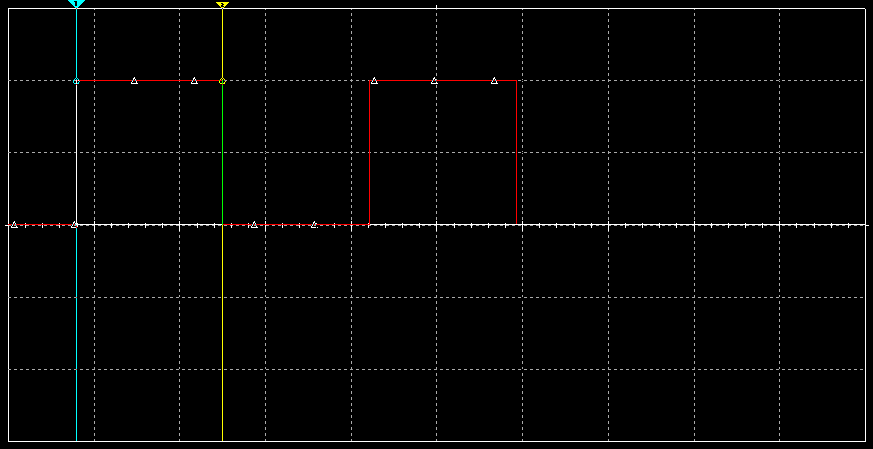
\includegraphics[width=0.36\linewidth]{images/simulation-oscillator.png}
    }
    \quad
    \subfigure[分频器]{
        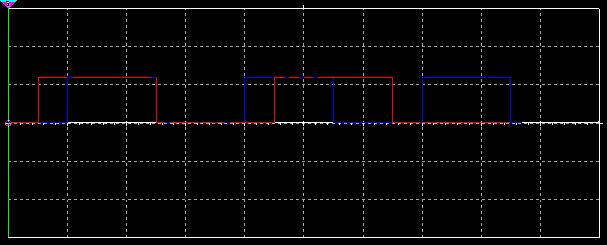
\includegraphics[width=0.46\linewidth]{images/simulation-freq-divider.png}
    }
    \\
    \subfigure[滤波器]{
        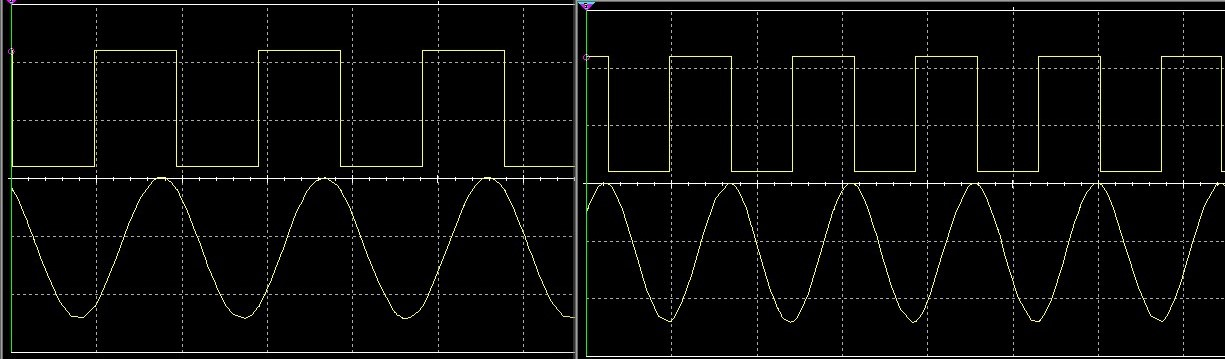
\includegraphics[width=0.9\linewidth]{images/simulation-filter.jpg}
    }
    \\
    \subfigure[移相器]{
        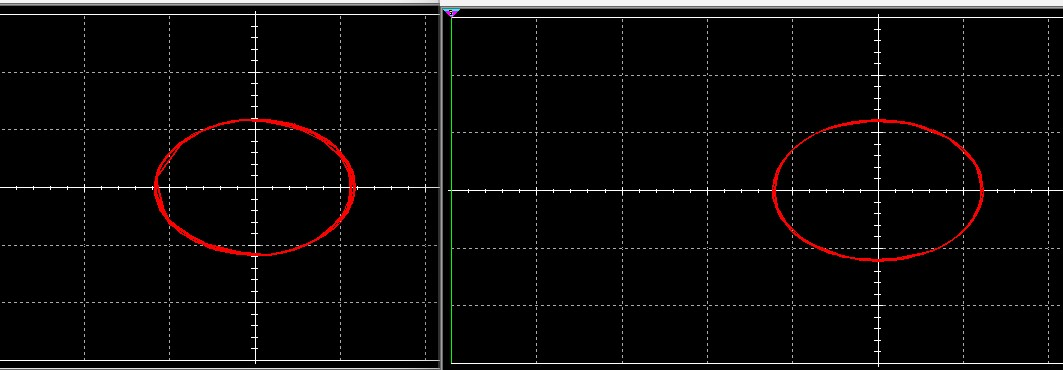
\includegraphics[width=0.53\linewidth]{images/simulation-phase-shifter.jpg}
    }
    \quad
    \subfigure[最终级联]{
        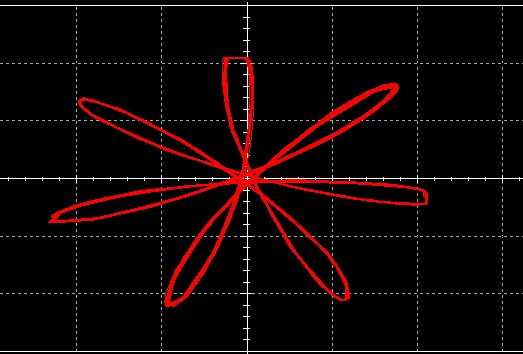
\includegraphics[width=0.28\linewidth]{images/simulation-whole.jpg}
    }
    \caption{仿真结果}
    \label{plot:multi-1}
\end{figure}
最终波形略有失真,分析原因可能是滤波器输出波形不是严格的正弦波;同时也无法确保两路的输出波形振幅完全相同,实验中滤波器和移相器均使用微调电阻使输出波形为正弦波形,且振幅接近,以最大程度减少失真。



\section{实验数据整理和分析}
我们依次对各个模块进行了级联测试,在确定了之前模块功能正常后接入新的模块,中间步骤没有拍照。
\par
振荡器和分频器产生的波形均为比较好的方波,经过滤波器后,产生的正弦波有轻微的毛刺,经过移相器后使用示波器的XY模式能得到非常好的圆形,加法器工作正常。
\begin{figure}[H]
    \centering
    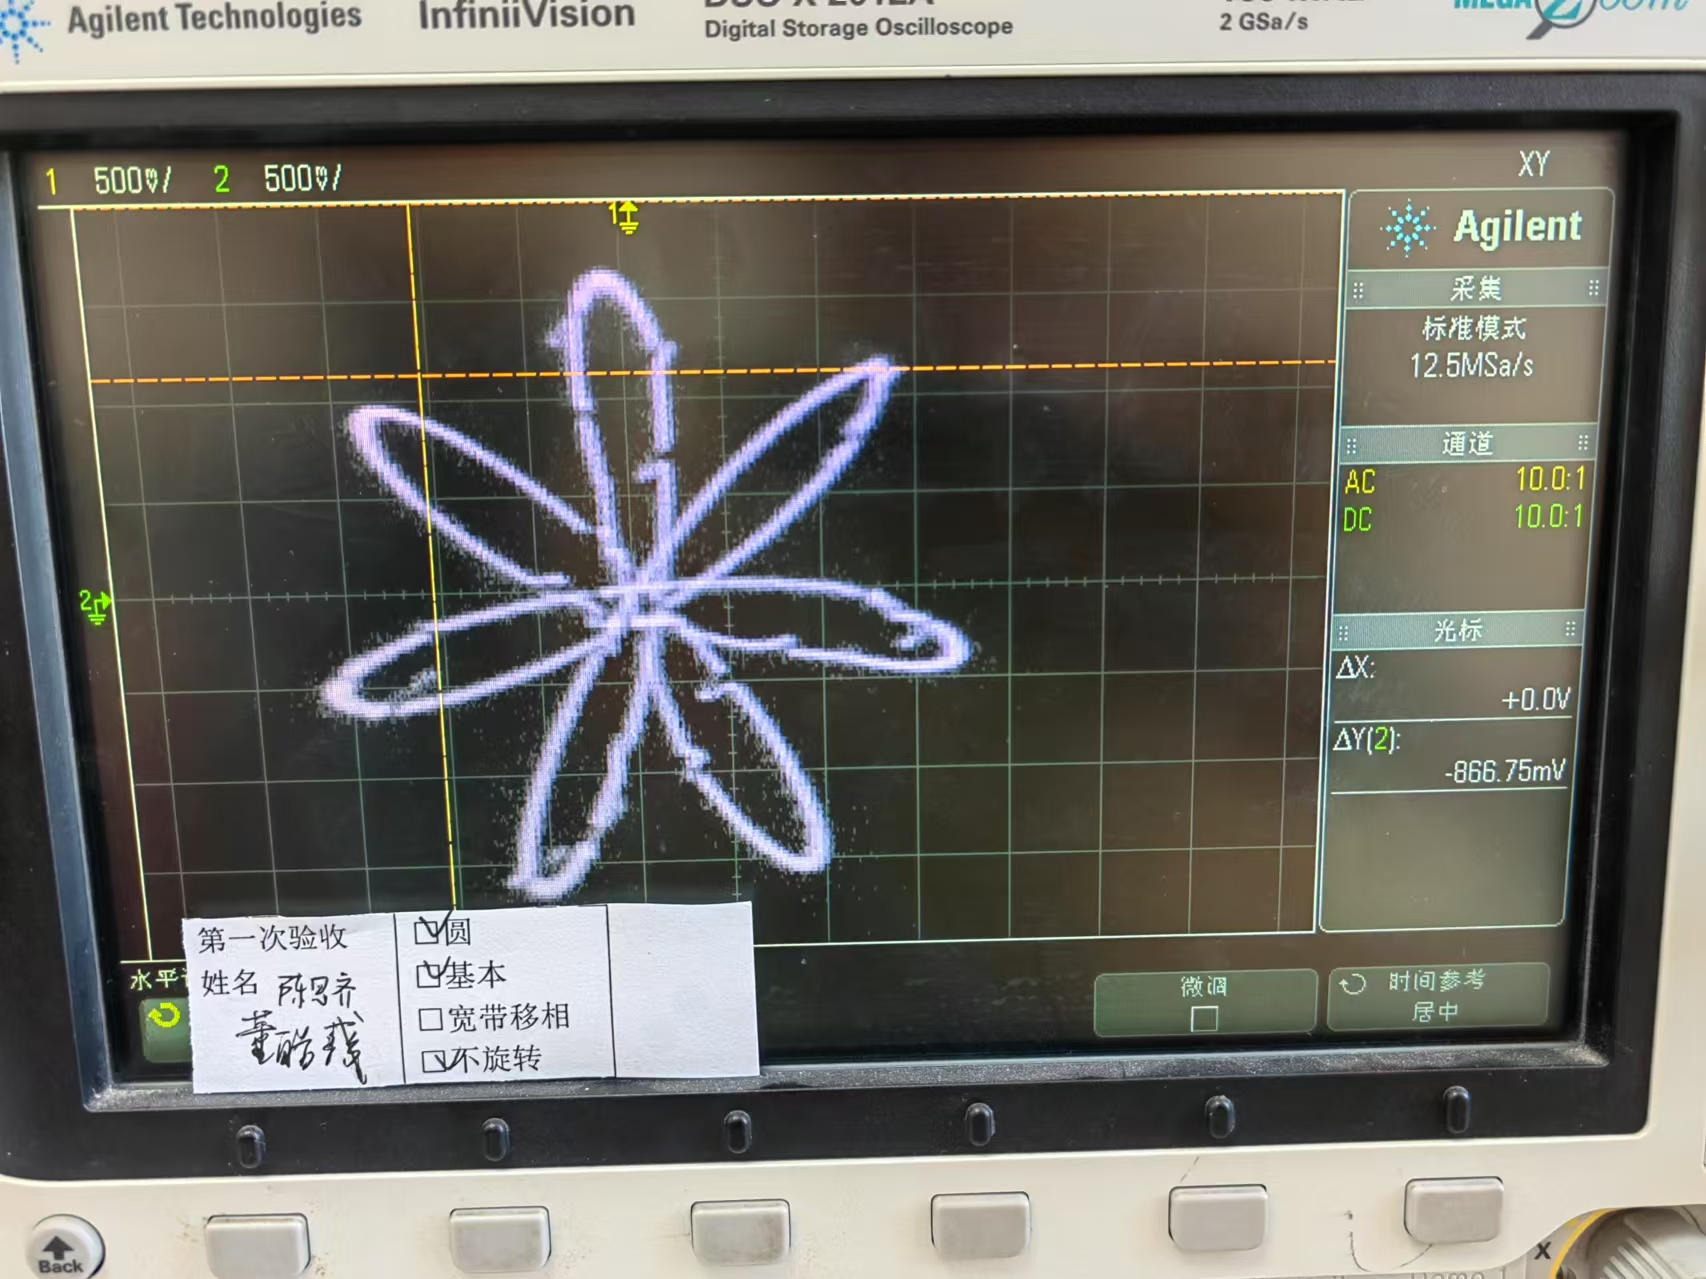
\includegraphics[width=0.8\linewidth]{images/result.jpg}
    \caption{最终实验结果}
    \label{plot:final-result}
\end{figure}
输出的万花尺图案与仿真结果基本一致,但有毛刺现象.
\par
原因分析:一方面可能是滤波器滤波不干净,有一小部分高频分量通过了滤波器;另一方面可能是实际电路搭建的时候走线比较乱,各个元件相互交叉,可能产生了寄生效应。

\section{实验总结}
实验完成的一波三折,其实在第一次来的时候大部分电路都搭好了,但滤波器因为没有在输入的时候接入一个大电阻,导致输出一直是方波,无法实现滤波功能,调节了两节课多,甚至把滤波器拆了重新搭了一次,终于在第二次的最后找到了错误,在第三次实验的时候完成了实验。
\par
在调节滤波器的时候,双联电位器和 $ 50~\mathrm{k}\Omega $ 电位器都需要调节,一开始两个一起瞎调,后来发现双联电位器只与频率有关,所以应该先调节双联电位器使得滤波器输出的频率与输入相同,这时候停止给滤波器供电,调节50kΩ电位器使得电路刚好起振,这时再把50kΩ电位器调小一点,就正好使得振荡器变成滤波器且输出振幅较大了。
\par
通过这次实验,我对电路系统有了更深刻的认识,在搭建时不仅需要考虑各部分的功能,同时也要充分考虑级联之后的效果,各个功能电路之间可能的相互影响,这样才能保证系统的正常工作,在必要的时候也需要通过增加额外的元件减轻相互的影响;同时,我也对噪声有了更深刻的认识,可能最初的一点小误差经过后续的功能电路就会被放大,进而产生显著的影响,所以在设计电路的时候尽可能减小噪声很关键。



\appendix
\onecolumn

\section{电路原理图}
\begin{figure}[H]
    \centering
    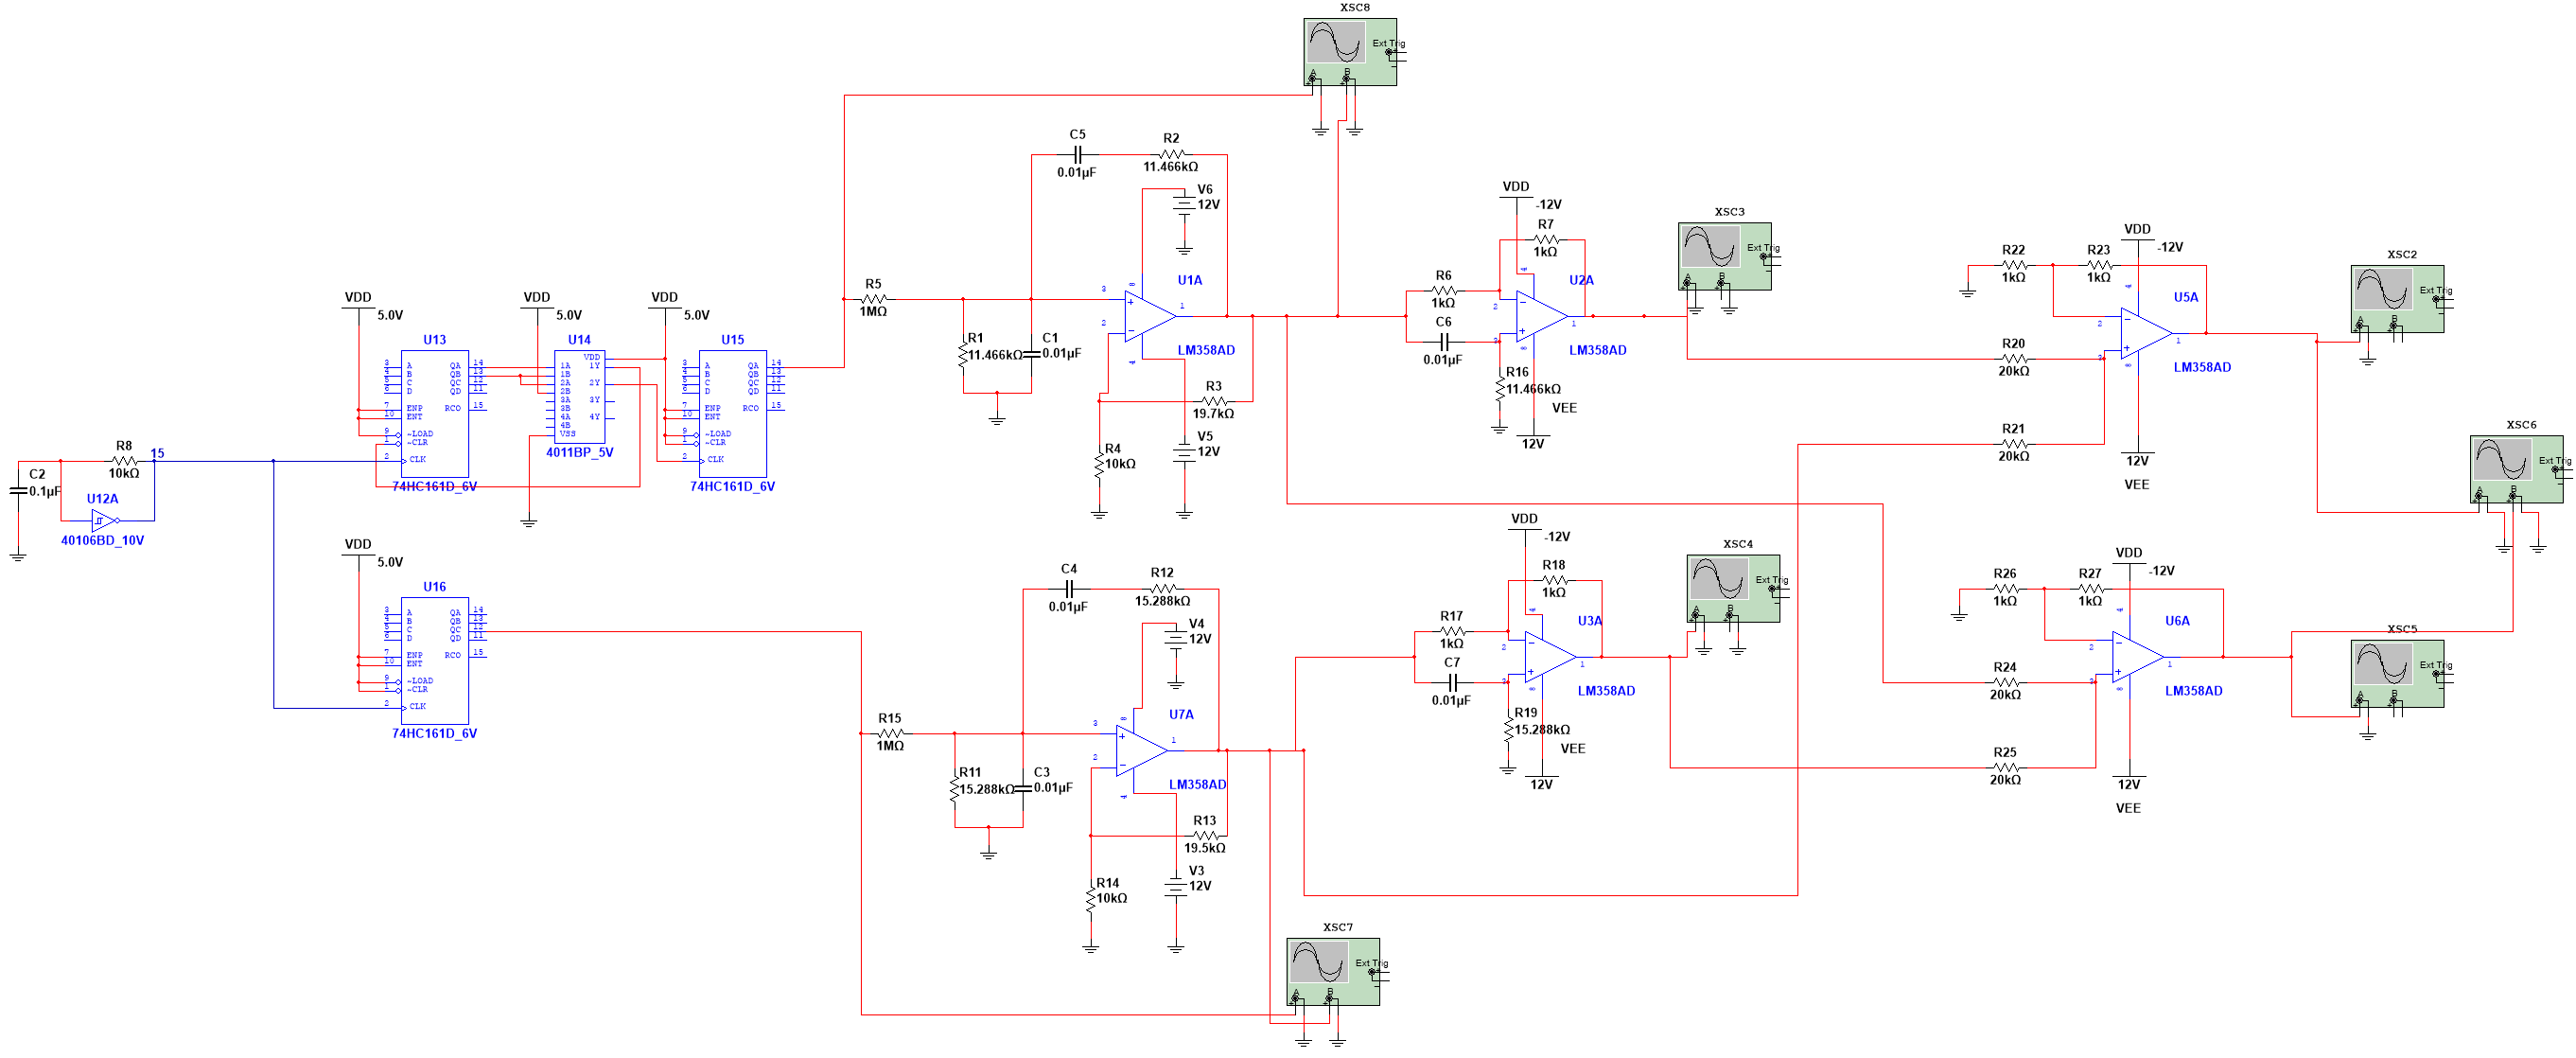
\includegraphics[width=1.2\linewidth,angle=-90]{images/circuit-full.png}
    \caption{电路原理图}
\end{figure}
多使用了一块面包板和一个74HC161芯片。



\section{示波器上呈现效果照片}
\begin{figure}[H]
    \centering
    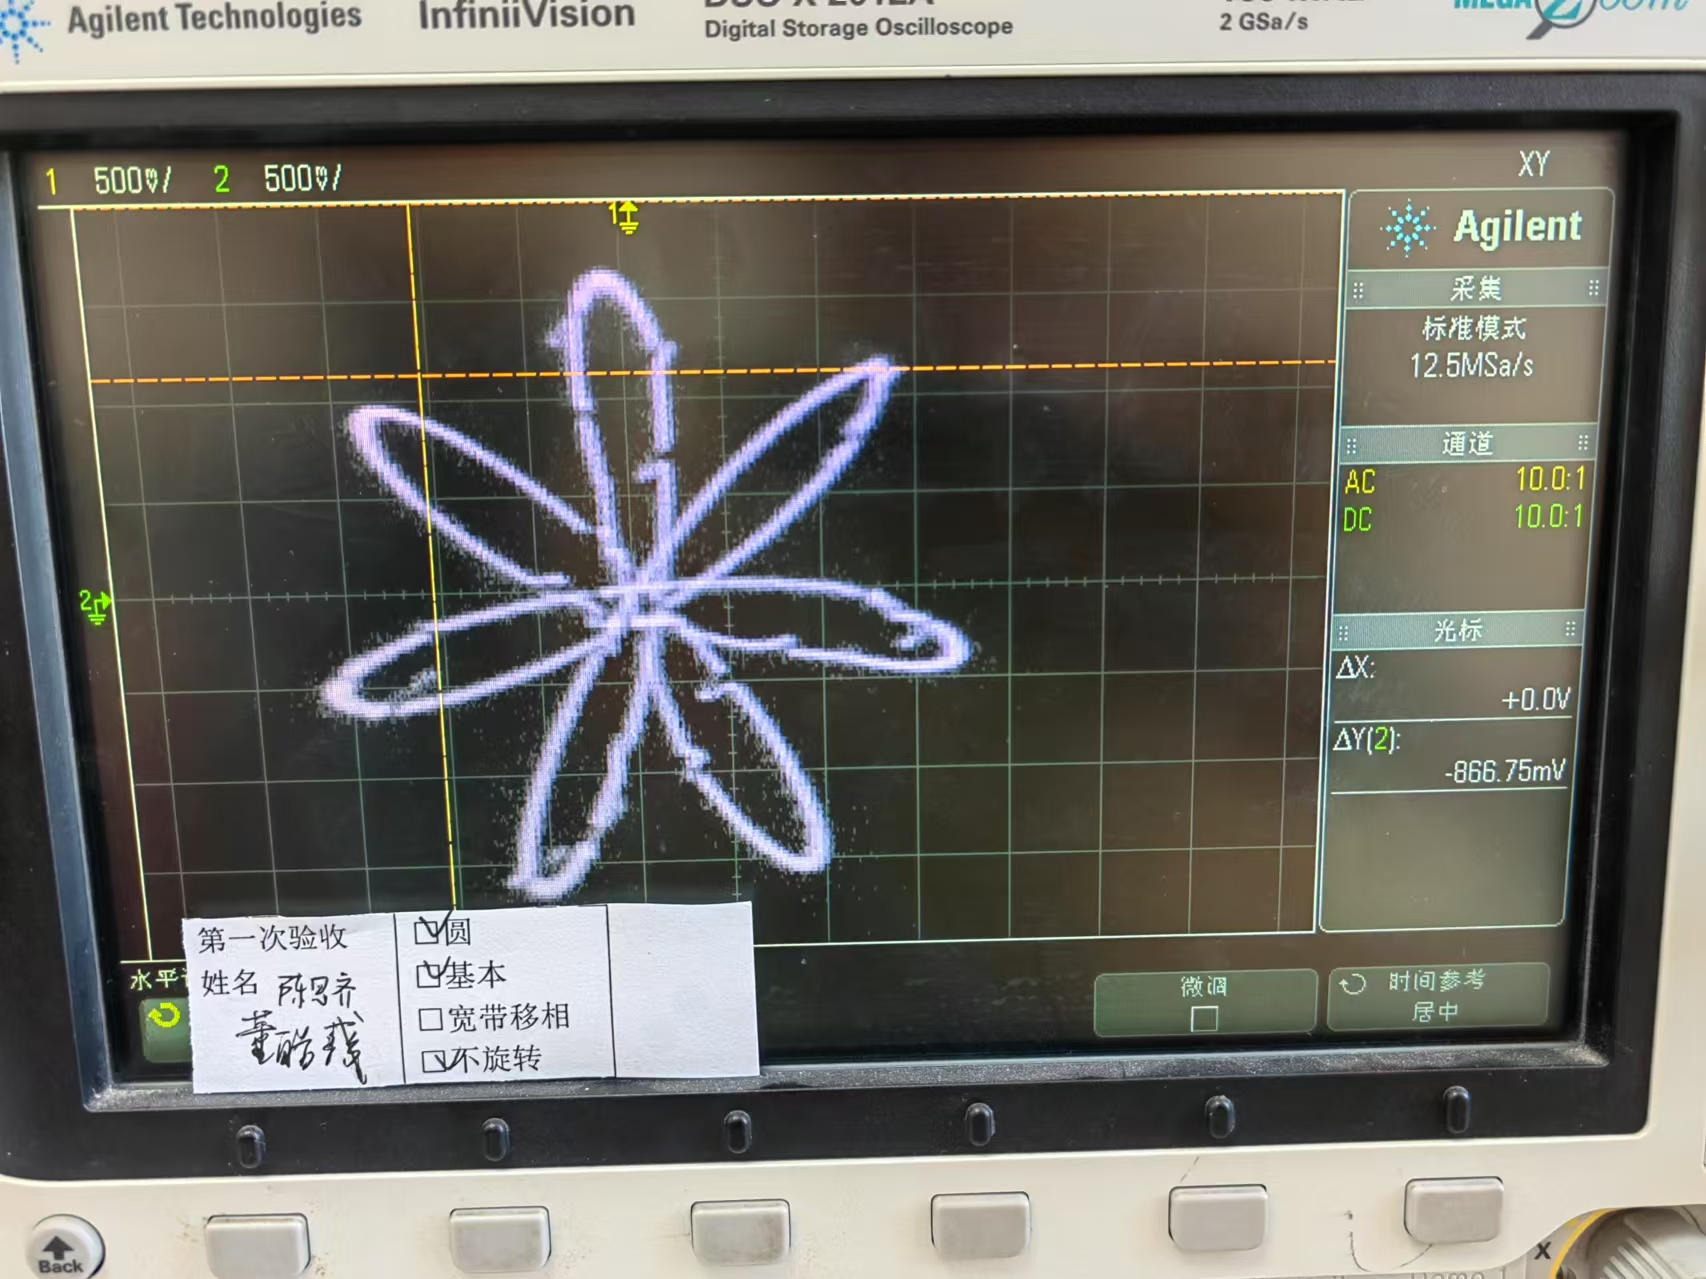
\includegraphics[width=0.6\linewidth]{images/result.jpg}
    \caption{最终万花尺图案}
\end{figure}
我们也尝试了其他的频率比(2:3),也得到了相应的图案。
\begin{figure}[H]
    \centering
    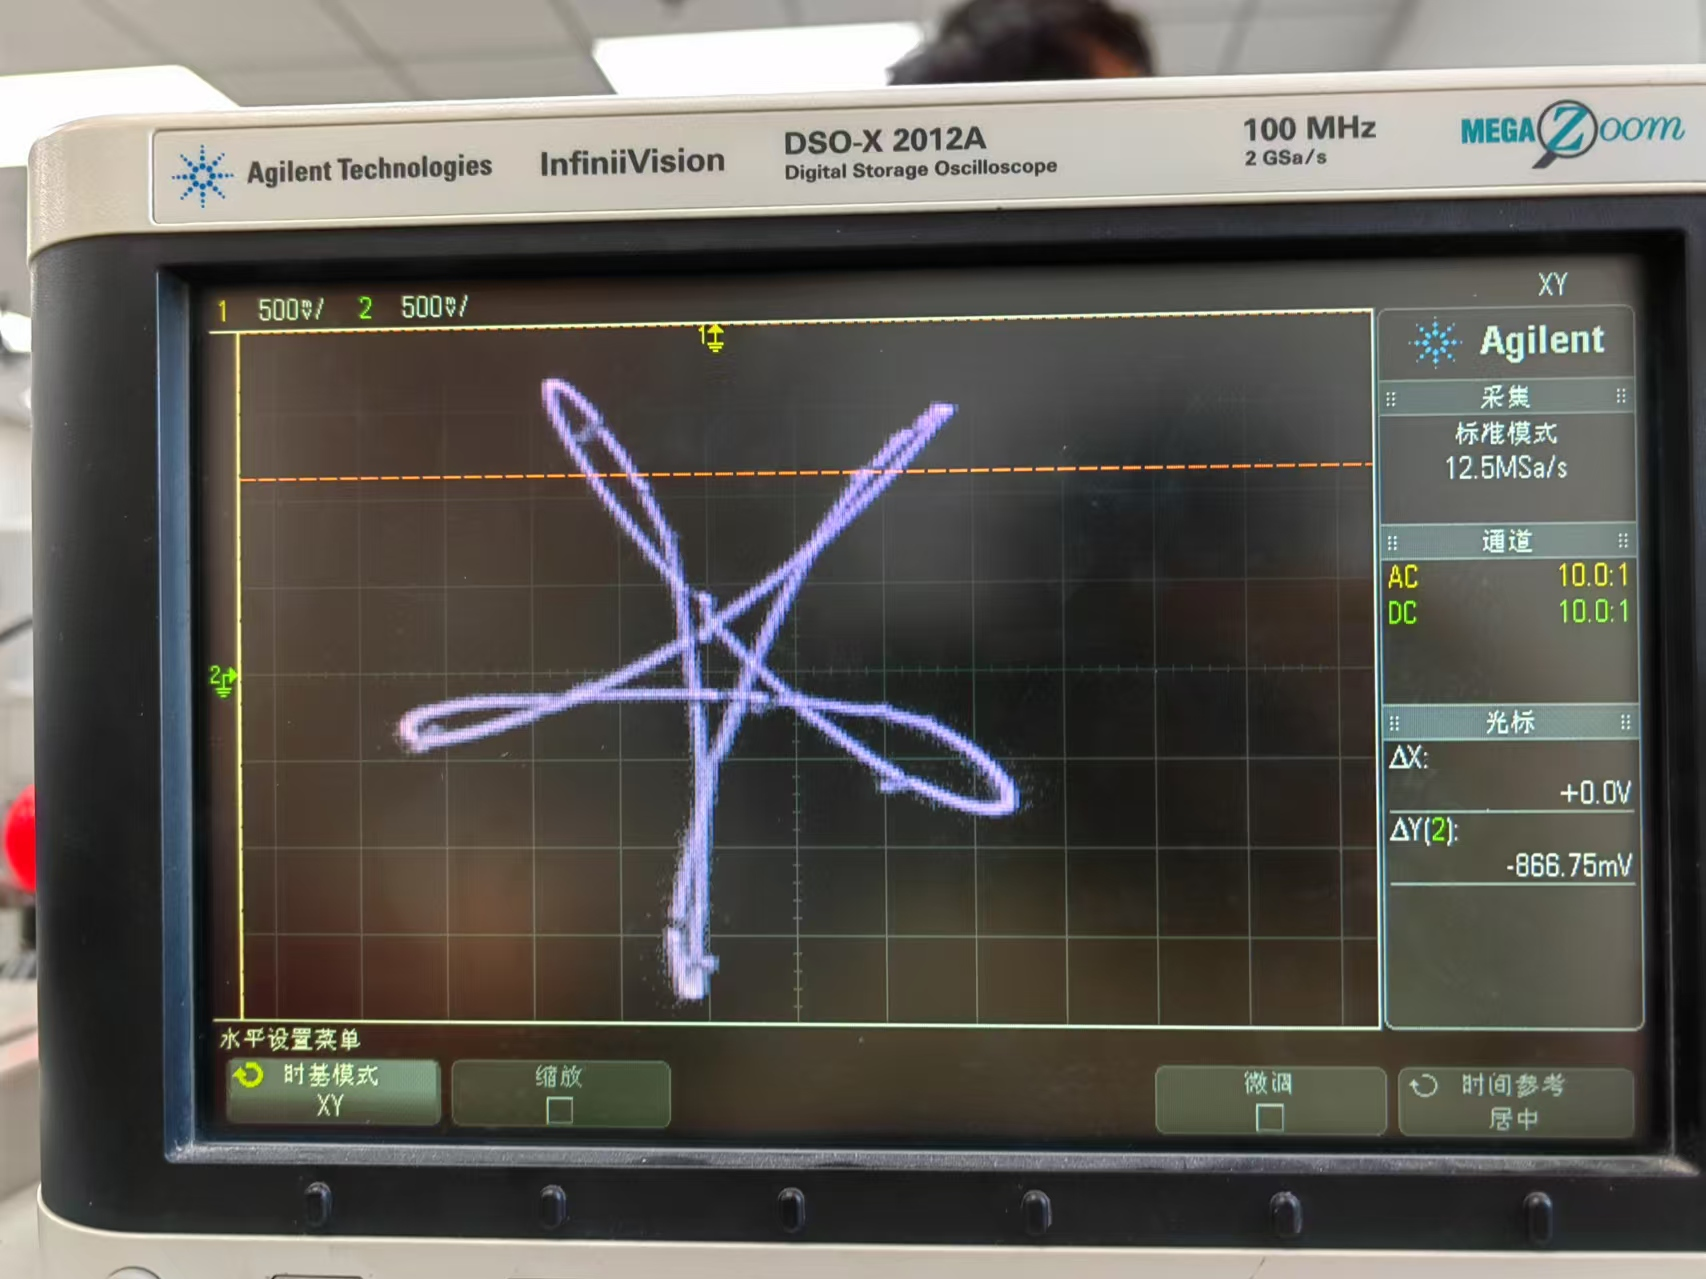
\includegraphics[width=0.6\linewidth]{images/result2.jpg}
    \caption{另一种万花尺图案}
\end{figure}



\section{电路整体照片}
\begin{figure}[H]
    \centering
    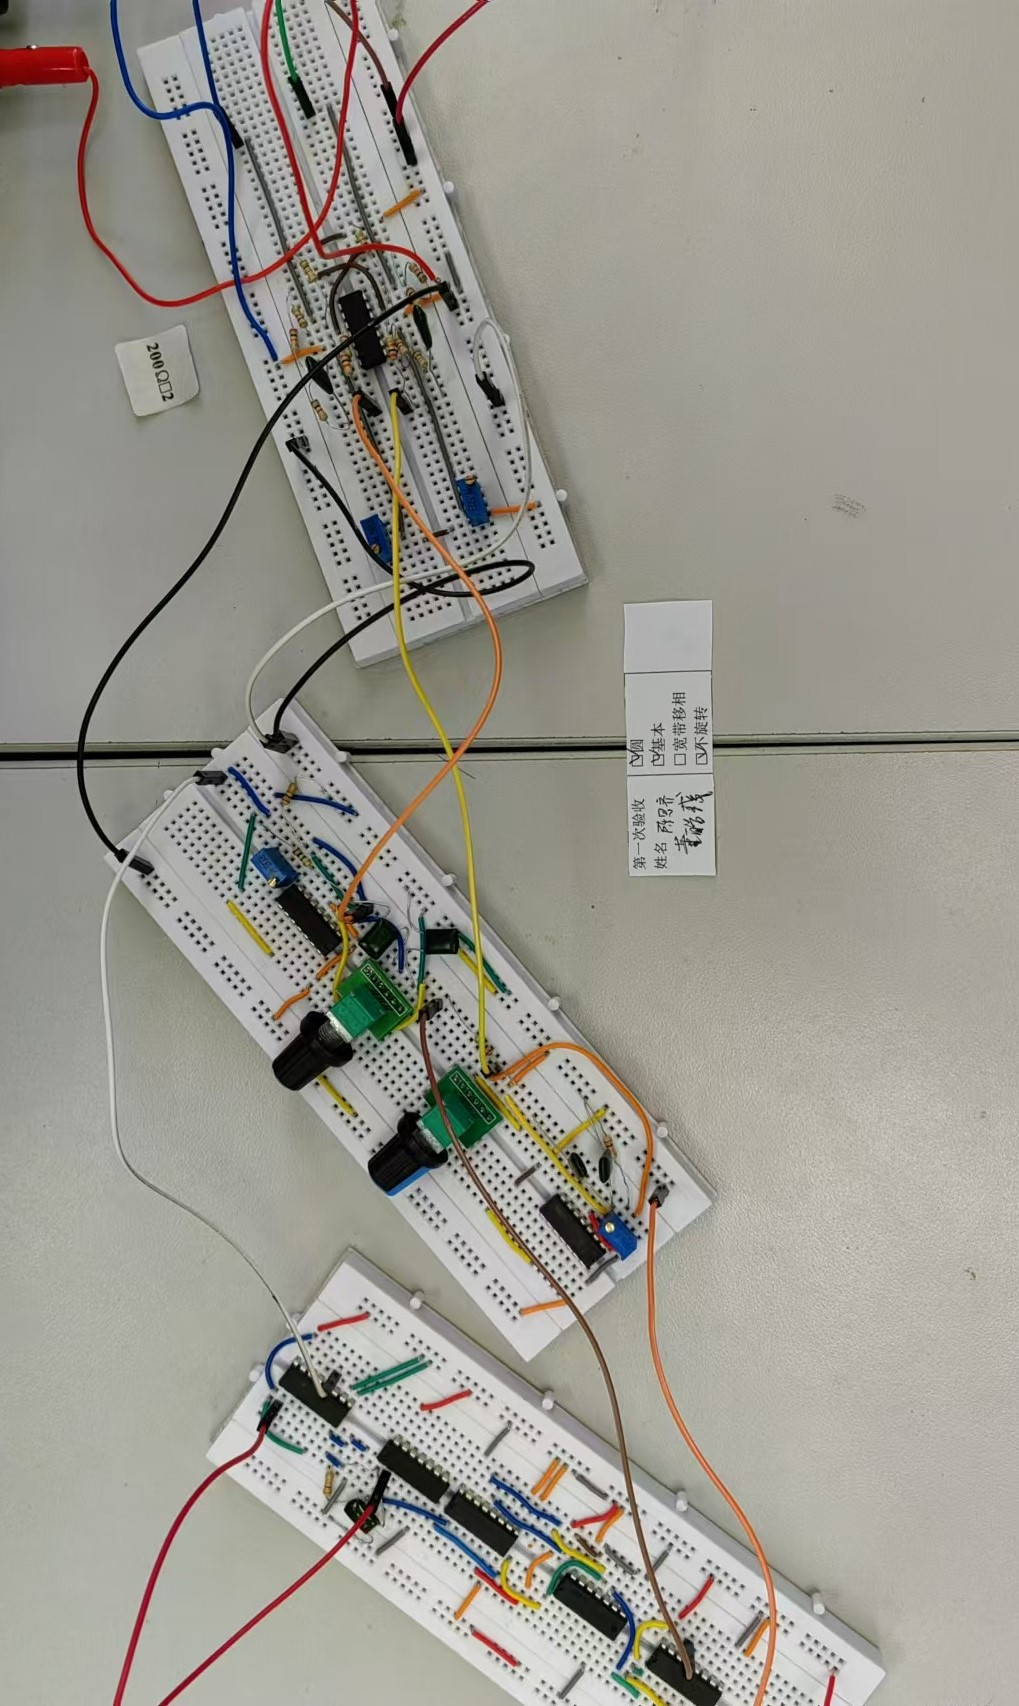
\includegraphics[width=0.7\linewidth]{images/circuit-real.jpg}
    \caption{实际电路图}
\end{figure}

\end{document}
